\documentclass[10pt, twocolumn]{article}

\usepackage{scrextend}
\changefontsizes{8pt}

\makeatletter
\renewcommand*{\fps@figure}{!htb}
\renewcommand*{\fps@table}{!htb}
\makeatother

\usepackage{sectsty}
\sectionfont{\fontsize{11}{11}\selectfont}
\subsectionfont{\fontsize{10}{11}\selectfont}

\usepackage[compact]{titlesec}
\titlespacing{\section}{0pt}{2ex}{1ex}
\titlespacing{\subsection}{0pt}{1ex}{1ex}
\titlespacing{\subsubsection}{0pt}{0.5ex}{1ex}

\setlength{\parskip}{0cm}
\setlength{\parindent}{1em}

\usepackage{geometry}
 \geometry{
 a4paper,
 total={170mm,257mm},
 left=20mm,
 top=20mm,
 }
\usepackage[utf8]{inputenc}
\usepackage[hidelinks]{hyperref}
\usepackage{amsmath, bm}
\usepackage[ruled,vlined]{algorithm2e}
\usepackage{amssymb}
\usepackage{graphicx}
\usepackage{float}
\usepackage{booktabs}
\usepackage[parfill]{parskip}
\usepackage{comment}
\usepackage{subcaption}
\usepackage{booktabs}



\usepackage{listings}
\lstset{
    language=Python,
    breaklines=true,
    breakatwhitespace=true,
    basicstyle=\footnotesize,
    frame=lines
}
\usepackage[capitalise, nameinlink]{cleveref}

\usepackage[sorting=none, style=verbose]{biblatex}
\addbibresource{lab_2.bib}

\usepackage{titling}
\setlength{\droptitle}{-1cm}

\title{\Large COMP6248 Lab 2 Exercise -- PyTorch Autograd}
\author{\small Wei Chien Teoh (Eugene)\\\bigskip \href{mailto:wct1c16@soton.ac.uk}{wct1c16@soton.ac.uk}}
\date{\small 29 April 2021}

\begin{document}

\maketitle

\section*{Introduction}

The results are seeded using \lstinline{torch.manual_seed(0)} to provide reproducible results.

\section{Implement matrix factorisation using gradient descent (take 2)}

\subsection{Implement gradient-based factorisation using PyTorch's AD}

\begin{lstlisting}
from typing import Tuple
import torch
import torch.nn.functional as F

def gd_factorise_ad(A: torch.Tensor, rank: int, num_epochs=1000, lr=0.01) -> Tuple[torch.Tensor, torch.Tensor]:
    m, n = A.shape
    U = torch.rand((m, rank), requires_grad=True)
    V = torch.rand((n, rank), requires_grad=True)

    for epoch in range(num_epochs):
        
        U.grad, V.grad = None, None

        loss = F.mse_loss(A, U @ V.T, reduction='sum')

        loss.backward()

        U.data -= lr * U.grad
        V.data -= lr * V.grad

    return U, V

\end{lstlisting}

\subsection{Factorise and compute reconstruction error on real data}

The results for both gradient-based matrix factorisation (MF) and truncated SVD are shown below.

\begin{align*}
    \begin{split}
        \text{GD Loss} &= 15.228897094726562\\
        \text{Truncated Loss} &= 15.22883415222168
    \end{split}
\end{align*}

Both results are almost identical. GD factorisation performs gradient-based minimisation on the Frobenius norm. Truncated SVD directly performs low-rank approximation by reducing the SVD to rank 2.

\subsection{Compare against PCA}

\begin{figure}
    \centering
    \begin{subfigure}{.7\linewidth}
        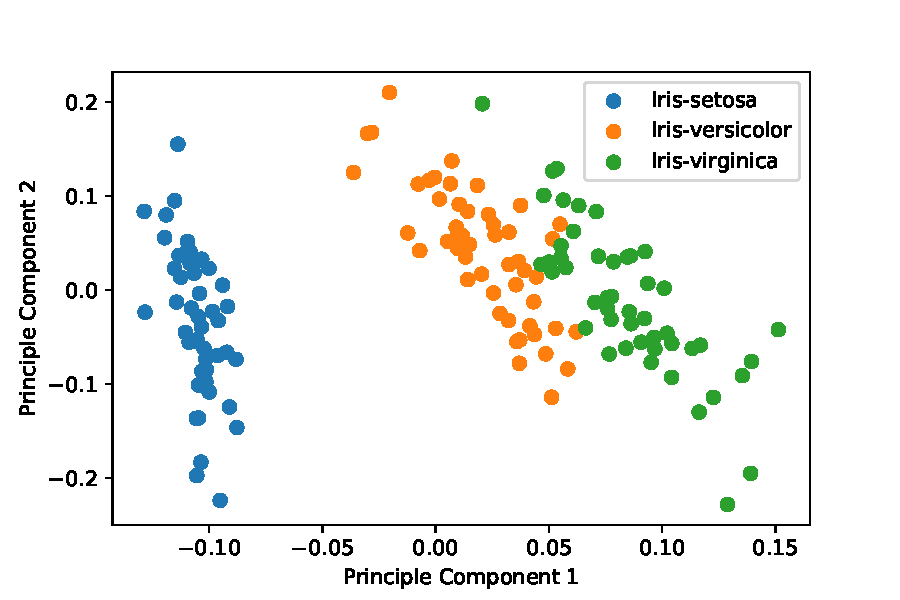
\includegraphics[width=\linewidth]{Figures/pca_svd.pdf} 
        \caption{SVD}
        \label{fig:svd}
    \end{subfigure}
    \begin{subfigure}{.7\linewidth}
        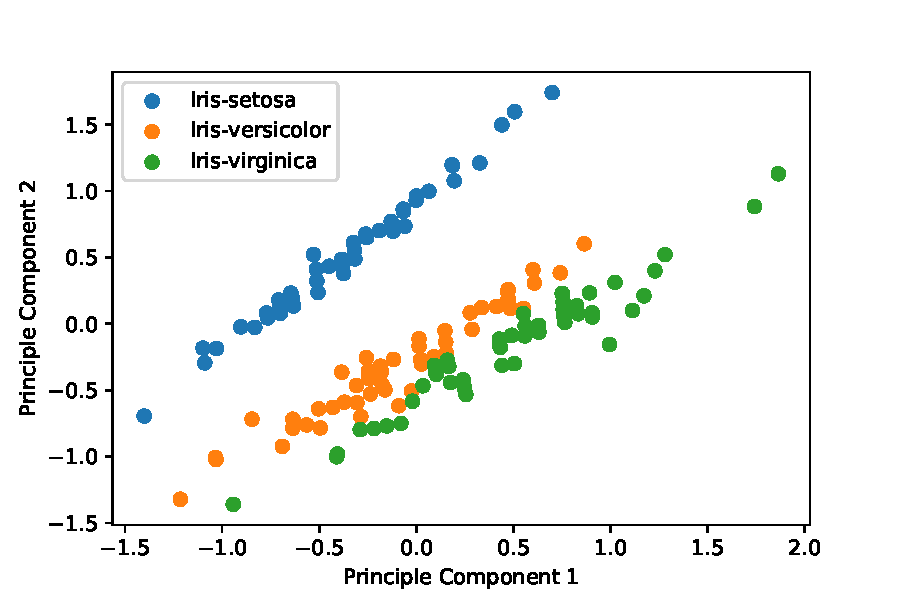
\includegraphics[width=\linewidth]{Figures/pca_gd.pdf} 
        \caption{Matrix Factorisation}
        \label{fig:mf}
    \end{subfigure}
    \caption{Projections of first two principle components.}
\end{figure}

The principle components computed by SVD, $\pmb{U}_t$ and by MF, $\hat{\pmb{U}}$ are illustrated in \cref{fig:svd} and \cref{fig:mf} respectively. $\hat{\pmb{U}}$ is observed to be a rotated and scaled version of $\pmb{U}_t$. As such, maximising variance is analogous to minimising reconstruction error.

\section{A simple MLP}

\subsection{Implement the MLP}

\begin{lstlisting}
def mlp(data, W1, W2, b1, b2):
    return torch.relu(data @ W1 + b1) @ W2 + b2

def train_mlp(data_tr: torch.Tensor, targets_tr: torch.Tensor, num_epochs: int = 100, lr: int = 0.01):
    # initialise weights and biases
    W1 = torch.rand((4, 12), requires_grad=True)
    W2 = torch.rand((12, 3), requires_grad=True)
    b1 = torch.rand(1, requires_grad=True)
    b2 = torch.rand(1, requires_grad=True)

    for epoch in range(num_epochs):
        logits = mlp(data_tr, W1, W2, b1, b2)
        loss = torch.nn.functional.cross_entropy(
            logits, 
            targets_tr, 
            reduction="sum")
        loss.backward()

        # update weights
        with torch.no_grad():
            W1 -= lr * W1.grad
            W2 -= lr * W2.grad
            b1 -= lr * b1.grad
            b2 -= lr * b2.grad

        for params in [W1, W2, b1, b2]:
            params.grad.zero_()

    return W1, W2, b1, b2
\end{lstlisting}

\subsection{Test the MLP}

% \begin{figure}
%     \centering
%     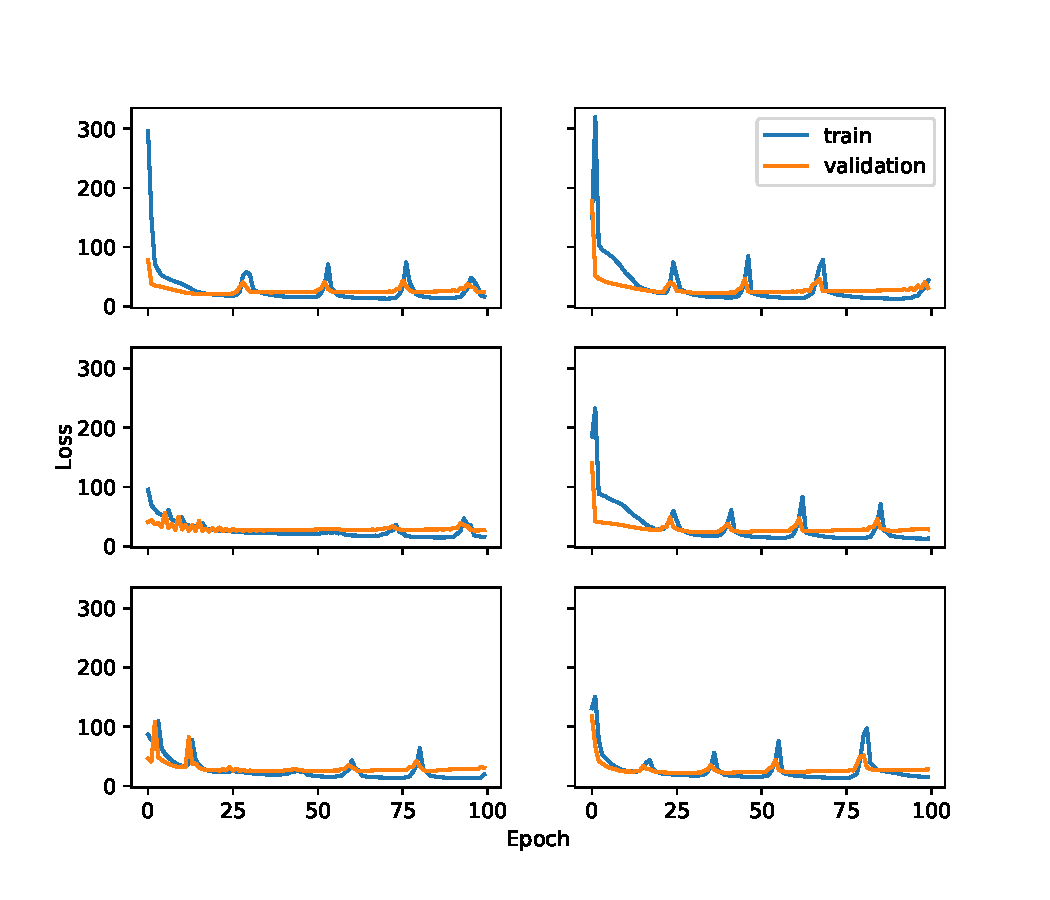
\includegraphics[width=\linewidth]{Figures/loss_curves.pdf}
%     \caption{Loss curves of repeated MLP training.}
%     \label{fig:loss-curves}
% \end{figure}

\begin{table}
    \centering
    \caption{Accuracies of repeated MLP training.}
    \label{tab:accs}
    \begin{tabular}{lrr}
    \toprule
    \# &  Training Accuracy &  Validation Accuracy \\
    \midrule
    0 &               0.92 &                 0.88 \\
    1 &               0.66 &                 0.66 \\
    2 &               0.92 &                 0.88 \\
    3 &               0.71 &                 0.70 \\
    4 &               0.92 &                 0.88 \\
    5 &               0.92 &                 0.88 \\
    6 &               0.88 &                 0.82 \\
    7 &               0.95 &                 0.88 \\
    8 &               0.85 &                 0.90 \\
    9 &               0.77 &                 0.72 \\
    \bottomrule
    \end{tabular}
\end{table}

\cref{tab:accs} shows the results of the repeated MLP training. It is observed that bad random initialisation of weights and biases may majorly impact the accuracy. Examples of bad initialisation are experiments \#1, \#3 and \#9. This may be caused by being stuck at a bad local minima or the vanishing gradient problem. The latter might be due to the weights being initialised between the values 0 to 1.


\end{document}